\documentclass[11pt,a4paper]{article}

\usepackage[spanish,es-noquoting]{babel}
\usepackage[utf8]{inputenc}
\usepackage[T1]{fontenc}
\usepackage{lmodern}
\usepackage{geometry}
\usepackage{booktabs}
\usepackage{tabularx}
\usepackage{longtable}
\usepackage{array}
\usepackage{multirow}
\usepackage{float}
\usepackage{graphicx}
\usepackage{enumitem}
\usepackage{hyperref}
\usepackage{xcolor}
\usepackage{colortbl}
\usepackage{fancyhdr}

\geometry{margin=2.5cm}
\setlength{\parskip}{0.5em}
\setlength{\parindent}{0pt}
\hypersetup{colorlinks=true, linkcolor=black, urlcolor=blue}

\definecolor{malignored}{RGB}{231,76,60}
\definecolor{benigngreen}{RGB}{46,204,113}
\definecolor{lightgray}{RGB}{245,245,245}
\definecolor{bestrow}{RGB}{212,239,223}

\setlength{\headheight}{14pt}
\pagestyle{fancy}
\fancyhf{}
\lhead{\textit{Proyecto 2 -- Data Mining}}
\rhead{\textit{Informe Final Integrado (Semanas 1--4)}}
\cfoot{\thepage}
\renewcommand{\headrulewidth}{0.4pt}

\title{\textbf{Proyecto 2 -- Data Mining}\\[0.4em]
       \large Informe Final Integrado (Semanas 1--4)\\[0.2em]
       \normalsize Detección de Cáncer de Mama: Wisconsin Breast Cancer Dataset}
\author{Javier España \and Ángel Esquit \and Roberto Barreda \and Diego López}
\date{Abril 2026}

\begin{document}

\maketitle
\thispagestyle{empty}

\begin{center}
\large Universidad del Valle de Guatemala\\[0.2em]
\normalsize Curso: Data Mining\\[0.2em]
Problema: Clasificación binaria de tumor mamario (2 = Benigno, 4 = Maligno)
\end{center}

\vspace{0.5em}\hrule\vspace{1em}

\tableofcontents
\newpage

% ─────────────────────────────────────────────
\section{Resumen ejecutivo}
% ─────────────────────────────────────────────

Este proyecto de Data Mining desarrolló, validó y seleccionó un modelo de clasificación binaria para apoyo diagnóstico de cáncer de mama. Se utilizó el Wisconsin Breast Cancer Dataset con 675 muestras y 9 variables citológicas.

\textbf{Resultado final:} Selección de \textbf{SVM optimizado con kernel RBF en Escenario A} (todas las 9 variables).

\textbf{Desempeño alcanzado en test set:}
\begin{itemize}[leftmargin=1.4cm]
\item \textbf{Recall de clase maligna: 1.0000} (todos los malignos detectados)
\item \textbf{Falsos negativos: 0} (máxima seguridad clínica)
\item \textbf{Verdaderos positivos: 47/47} (sensibilidad perfecta)
\item \textbf{Precisión: 0.9038} (balance aceptable de especificidad)
\item \textbf{Accuracy general: 0.9630}
\end{itemize}

\textbf{Justificación de la selección:} En oncología, minimizar falsos negativos es crítico. El trade-off aceptado fue incrementar falsos positivos (5 casos) para garantizar cero omisiones de malignos. Este comportamiento es clínicamente defendible: evaluaciones adicionales son siempre preferibles a diagnósticos tardíos.

% ─────────────────────────────────────────────
\section{Introducción y contexto del problema}
% ─────────────────────────────────────────────

El cáncer de mama es una enfermedad oncológica prevalente con impacto significativo en pronostico y sobrevida. La detección temprana mediante análisis de rasgos citológicos es fundamental.

\subsection{Objetivo clínico y criterio de decisión}

El proyecto adoptó explícitamente una \textbf{prioridad clínica clara}: minimizar falsos negativos de la clase maligna, aceptando incremento controlado de falsos positivos si es necesario. Esto refleja el principio médico: ``mejor evaluar un caso benigno adicional que omitir un maligno''.

\subsection{Dataset: Wisconsin Breast Cancer Dataset}

\begin{itemize}[leftmargin=1.4cm]
\item \textbf{Tamaño original:} 683 registros, 11 columnas
\item \textbf{Variables predictoras:} 9 rasgos citológicos (escala 1--10)
\item \textbf{Variable objetivo:} \texttt{Class} (2=Benigno, 4=Maligno)
\item \textbf{Distribución original:} 65\% Benigno, 35\% Maligno (desbalance moderado 1.86:1)
\end{itemize}

% ─────────────────────────────────────────────
\section{Semana 1: Exploración y Análisis Exploratorio de Datos}
% ─────────────────────────────────────────────

\subsection{Objetivos de Semana 1}

Comprender la estructura del dataset, identificar patrones de separabilidad entre clases, detectar variables relevantes, y formular hipótesis que guíen el modelado.

\subsection{Hallazgos principales del EDA}

\begin{enumerate}[leftmargin=1.4cm]
\item \textbf{Separabilidad entre clases:} distribuciones claramente diferenciadas, especialmente en variables de uniformidad nuclear y tamaño celular.

\item \textbf{Variables más correlacionadas con \texttt{Class}:}
\begin{itemize}
\item Bare Nuclei (núcleos desnudos)
\item Uniformity of Cell Size (uniformidad de tamaño celular)
\item Uniformity of Cell Shape (uniformidad de forma celular)
\end{itemize}

\item \textbf{Colinealidad observada:} Correlación r=0.91 entre Uniformity of Cell Size y Uniformity of Cell Shape.

\item \textbf{Tratamiento de outliers:} se detectaron valores extremos (especialmente en casos malignos); se decidió mantenerlos por su valor diagnóstico.
\end{enumerate}

\subsection{Gráficas de EDA}

\begin{figure}[H]
\centering
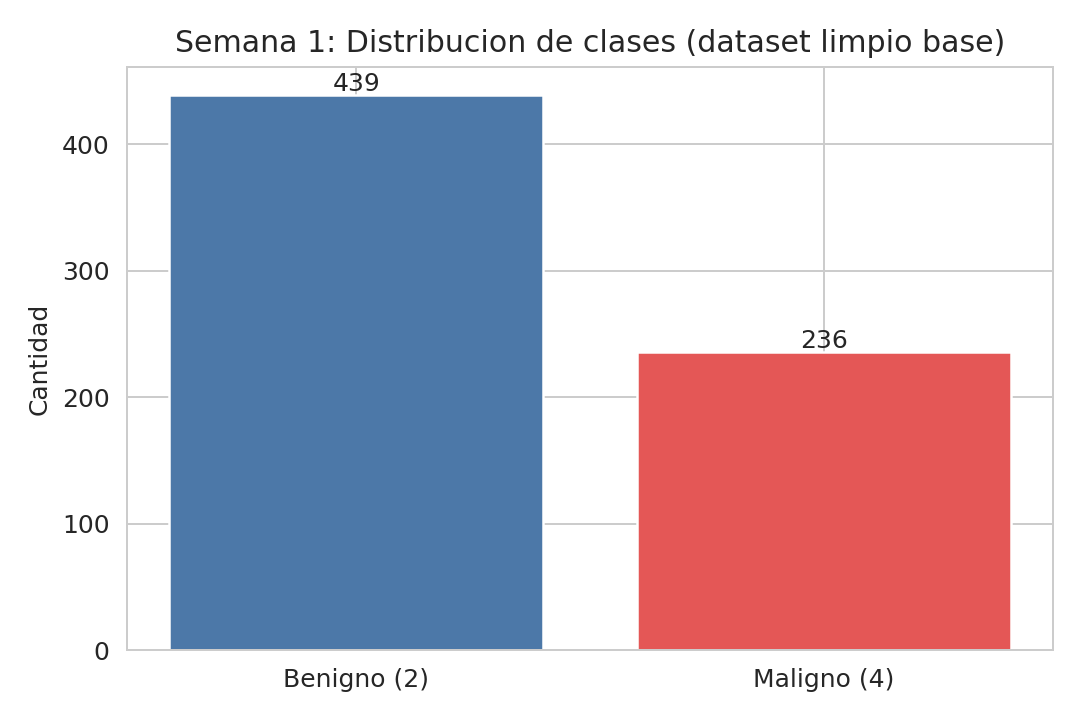
\includegraphics[width=0.9\textwidth]{figures/s1_distribucion_clases.png}
\caption{Distribución de clases en dataset limpio. Balance 65\% benignos vs. 35\% malignos.}
\label{fig:distribucion}
\end{figure}

\begin{figure}[H]
\centering
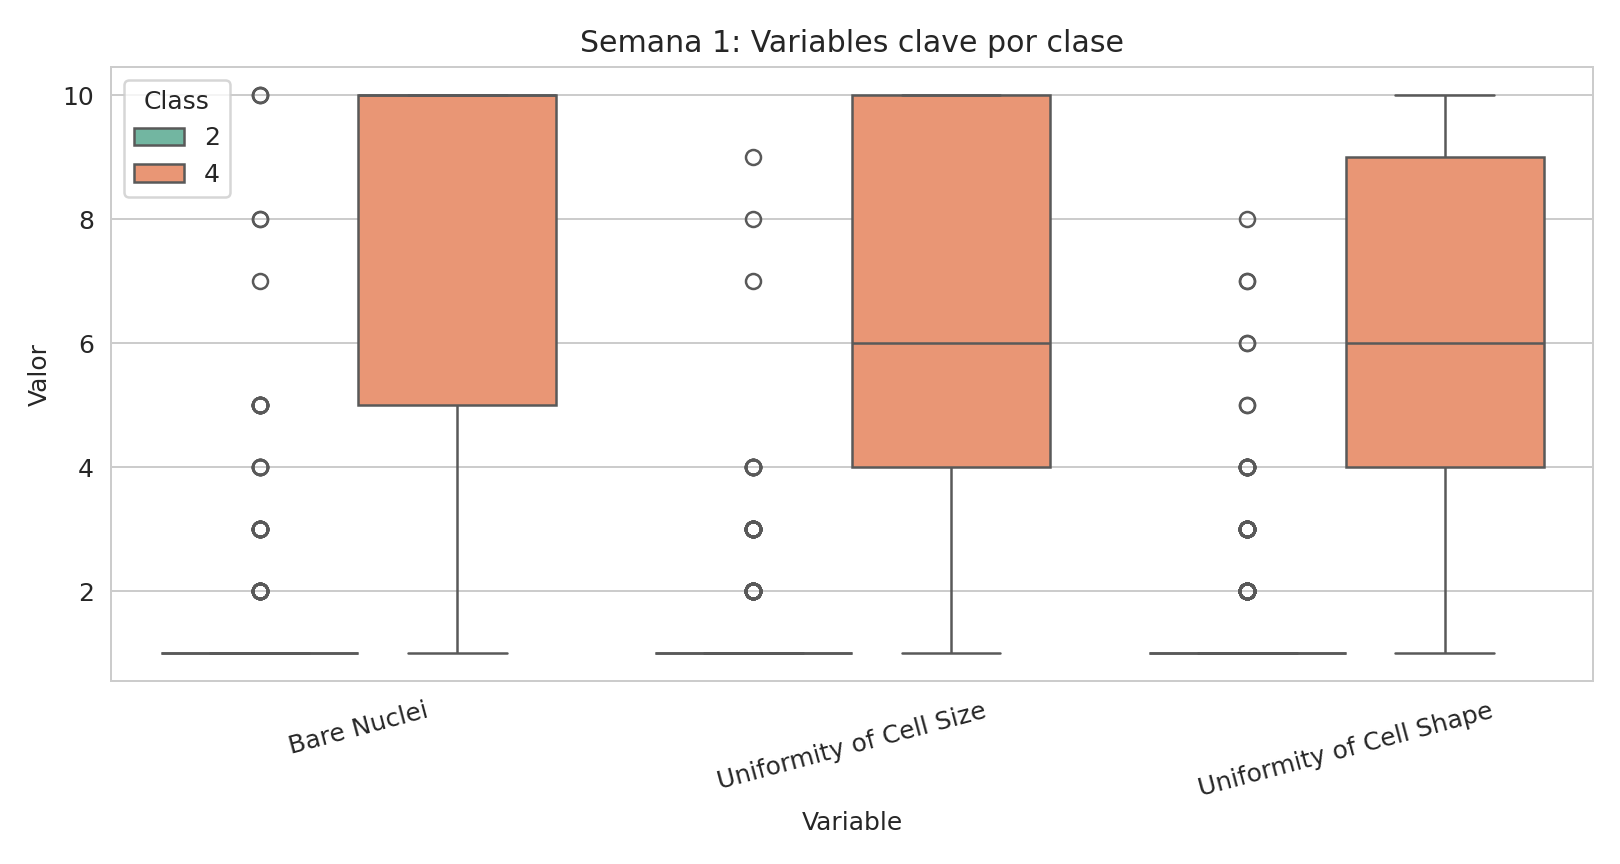
\includegraphics[width=0.9\textwidth]{figures/s1_boxplot_variables_clave.png}
\caption{Variables clave por clase. Diferenciación clara en núcleos y uniformidad celular.}
\label{fig:boxplot}
\end{figure}

\begin{figure}[H]
\centering
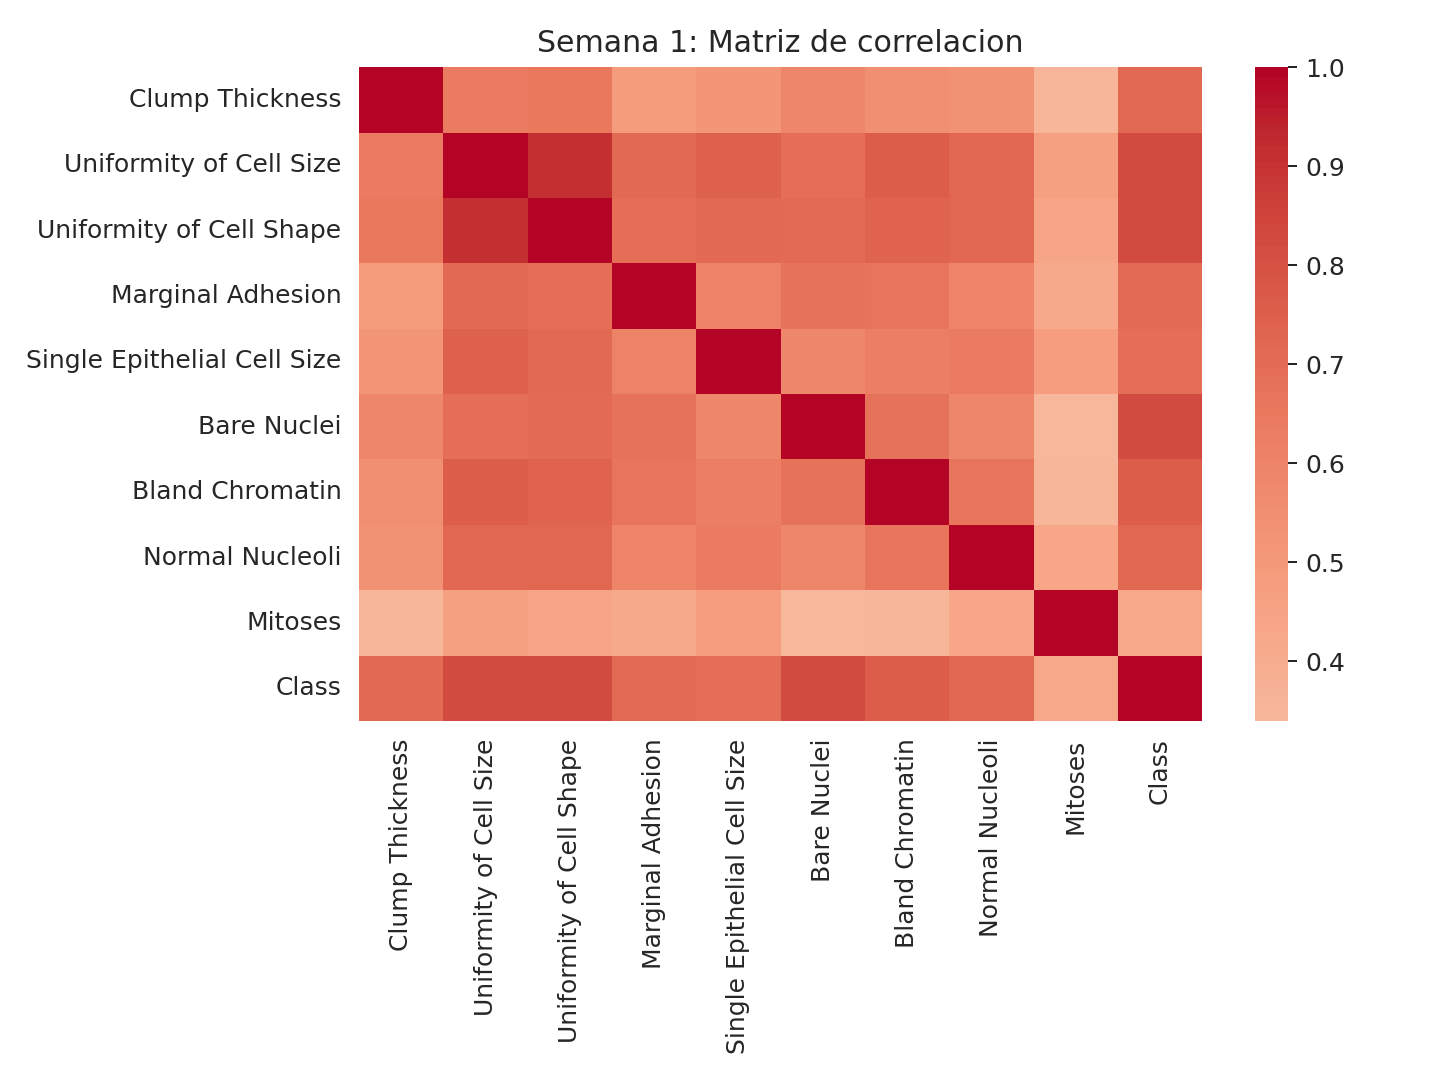
\includegraphics[width=0.9\textwidth]{figures/s1_correlacion_heatmap.png}
\caption{Matriz de correlación. Destaca colinealidad entre uniformidades y correlación de estas con Class.}
\label{fig:correlacion}
\end{figure}

\subsection{Hipótesis de trabajo formuladas}

Se establecieron 5 hipótesis que guiaron semanas posteriores:

\begin{table}[H]
\centering
\caption{Hipótesis de trabajo (Semana 1)}
\small
\renewcommand{\arraystretch}{1.2}
\begin{tabular}{lp{6cm}l}
\toprule
\textbf{H} & \textbf{Proposición} & \textbf{Verificación} \\
\midrule
H1 & Variables de uniformidad nuclear son críticas para separación & Semana 3: Confirmado \\
H2 & Modelos no lineales (SVM) superarán regresión logística & Semana 3: Confirmado \\
H3 & Recall maligna debe ser métrica principal & Semana 3: Adoptado \\
H4 & Colinealidad requiere prueba con subset de variables & Semana 2: Escenario B \\
H5 & Outliers deben conservarse por valor clínico & Semana 2: Aplicado \\
\bottomrule
\end{tabular}
\normalsize
\end{table}

% ─────────────────────────────────────────────
\section{Semana 2: Preparación de Datos y Modelos Base}
% ─────────────────────────────────────────────

\subsection{Limpieza de datos}

Se aplicaron transformaciones sistemáticas:

\begin{enumerate}[leftmargin=1.4cm]
\item \textbf{Conversión de tipos:} \texttt{Bare Nuclei} contenía valores \texttt{?} que fueron interpretados como nulos y tratados.
\item \textbf{Eliminación de duplicados exactos:} 8 registros idénticos fueron removidos.
\item \textbf{Exclusión de identificadores:} \texttt{Sample code number} fue excluido del modelado para evitar overfitting.
\end{enumerate}

\textbf{Resultado:}
\begin{itemize}[leftmargin=1.4cm]
\item \texttt{Datos\_limpio.csv}: 675 registros (con ID preservado)
\item \texttt{Datos\_modelado.csv}: 675 registros (sin ID, listo para ML)
\end{itemize}

\subsection{Diseño de escenarios}

Para probar robustez y abordar colinealidad:

\begin{table}[H]
\centering
\caption{Escenarios de experimentación}
\small
\renewcommand{\arraystretch}{1.2}
\begin{tabular}{lp{5cm}l}
\toprule
\textbf{Escenario} & \textbf{Descripción} & \textbf{Propósito} \\
\midrule
\rowcolor{bestrow}
A & Todas las 9 variables & Máxima información disponible \\
B & Top 3 variables (Bare Nuclei, Uniformities) & Test de robustez con subset \\
\bottomrule
\end{tabular}
\normalsize
\end{table}

\subsection{Partición entrenamiento/prueba}

\begin{table}[H]
\centering
\caption{Split del dataset (80/20 estratificado)}
\small
\renewcommand{\arraystretch}{1.15}
\begin{tabular}{lccc}
\toprule
& \textbf{Total} & \textbf{Train (80\%)} & \textbf{Test (20\%)} \\
\midrule
Benigno (2) & 440 & 286 & 88 \\
Maligno (4) & 235 & 154 & 47 \\
\midrule
\textbf{Total} & 675 & 540 & 135 \\
\bottomrule
\end{tabular}
\normalsize
\end{table}

\subsection{Modelos base entrenados}

Se entrenaron tres algoritmos sin optimización inicial:

\begin{enumerate}[leftmargin=1.4cm]
\item \textbf{Regresión Logística} (L2, default)
\item \textbf{K-Nearest Neighbors} (k=5, default)
\item \textbf{Support Vector Machine} (kernel RBF, default)
\end{enumerate}

\textbf{Desempeño base:} SVM mostró ventaja temprana en recall de clase maligna.

\subsection{Gráficas de Semana 2}

\begin{figure}[H]
\centering
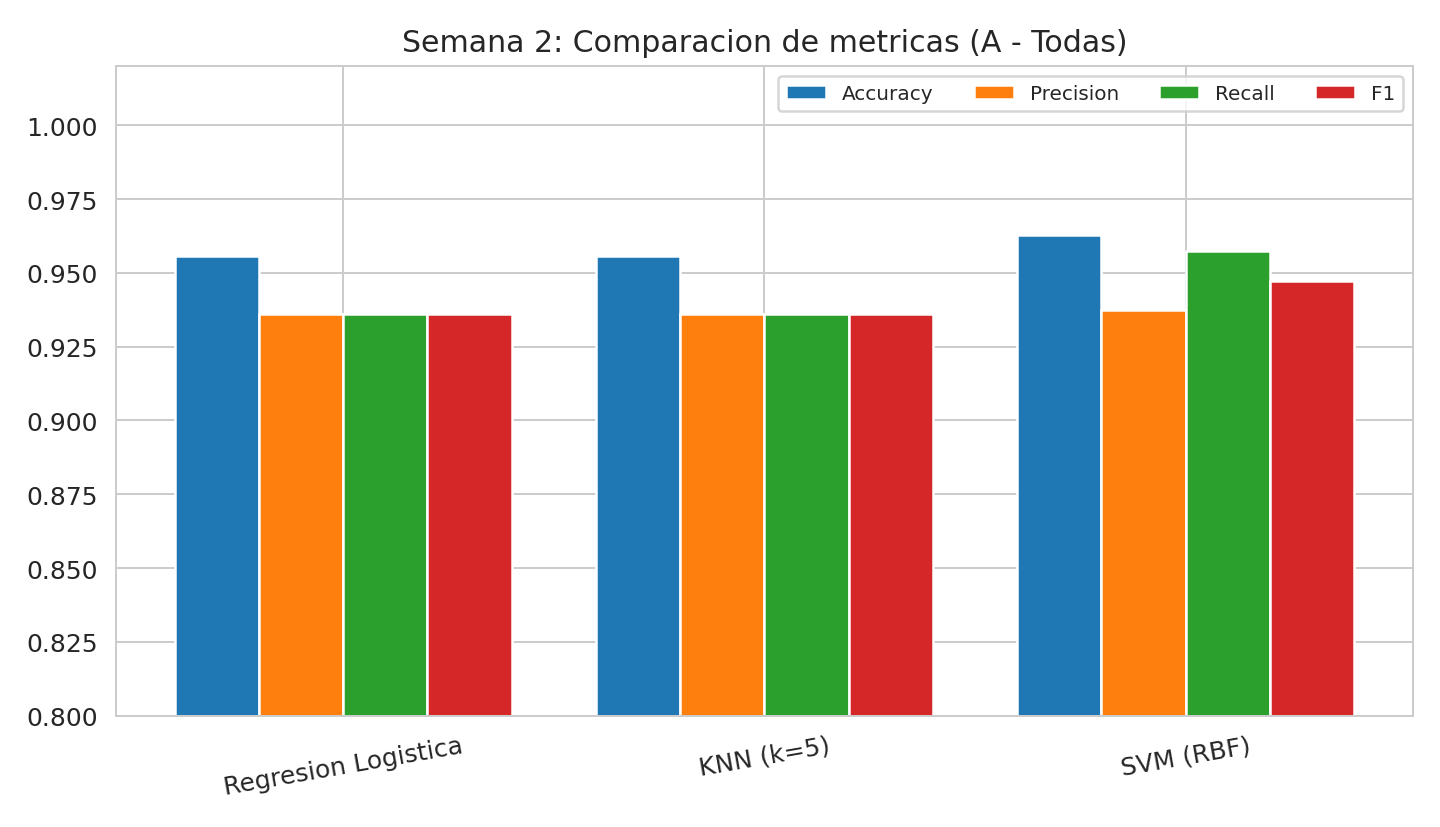
\includegraphics[width=0.9\textwidth]{figures/s2_metricas_A.png}
\caption{Métricas de modelos base en Escenario A (todas las variables).}
\label{fig:metricas_a}
\end{figure}

\begin{figure}[H]
\centering
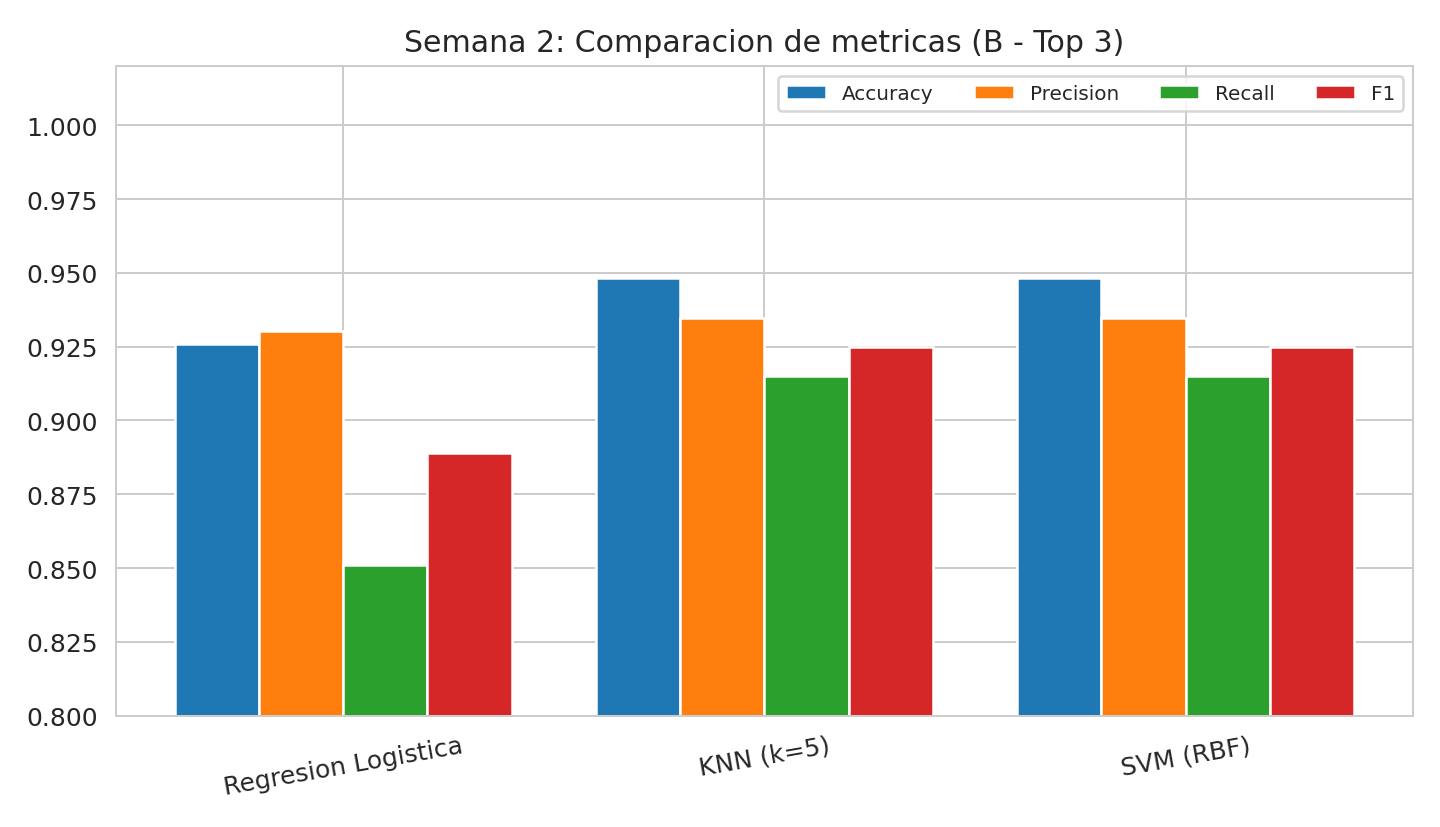
\includegraphics[width=0.9\textwidth]{figures/s2_metricas_B.png}
\caption{Métricas de modelos base en Escenario B (top 3 variables).}
\label{fig:metricas_b}
\end{figure}

% ─────────────────────────────────────────────
\section{Semana 3: Validación, Optimización y Selección Final}
% ─────────────────────────────────────────────

\subsection{Protocolo experimental}

Se implementó un protocolo riguroso de validación:

\begin{itemize}[leftmargin=1.4cm]
\item \textbf{Validación cruzada:} 5-Fold Stratified Cross-Validation
\item \textbf{Métrica de tuning:} Recall de clase maligna (maximizar)
\item \textbf{Escalado:} StandardScaler dentro de pipelines (sin data leakage)
\item \textbf{Optimización:} GridSearchCV para búsqueda de hiperparámetros
\end{itemize}

\subsection{Resultados de validación cruzada}

\textbf{Escenario A (todas las variables):}

\begin{table}[H]
\centering
\caption{CV resultados en Escenario A}
\small
\renewcommand{\arraystretch}{1.2}
\begin{tabular}{lcccc}
\toprule
\textbf{Modelo} & \textbf{Accuracy CV} & \textbf{Recall mal. CV} & \textbf{AUC CV} & \textbf{F1 CV} \\
\midrule
Regresión Logística (base) & 0.9704 & 0.9526 & 0.9941 & 0.9702 \\
KNN k=5 (base) & 0.9685 & 0.9472 & 0.9843 & 0.9684 \\
\rowcolor{bestrow}
SVM RBF (base) & 0.9611 & 0.9632 & 0.9898 & 0.9613 \\
\bottomrule
\end{tabular}
\normalsize
\end{table}

\textbf{Escenario B (top 3 variables):}

\begin{table}[H]
\centering
\caption{CV resultados en Escenario B}
\small
\renewcommand{\arraystretch}{1.2}
\begin{tabular}{lcccc}
\toprule
\textbf{Modelo} & \textbf{Accuracy CV} & \textbf{Recall mal. CV} & \textbf{AUC CV} & \textbf{F1 CV} \\
\midrule
Regresión Logística (base) & 0.9648 & 0.9366 & 0.9912 & 0.9647 \\
\rowcolor{bestrow}
KNN k=5 (base) & 0.9667 & 0.9525 & 0.9823 & 0.9667 \\
SVM RBF (base) & 0.9574 & 0.9418 & 0.9880 & 0.9575 \\
\bottomrule
\end{tabular}
\normalsize
\end{table}

\subsection{Resultados tras optimización de hiperparámetros}

\textbf{Comparación final: Modelos optimizados en test set}

\begin{table}[H]
\centering
\caption{Resumen de modelos optimizados (test set)}
\small
\renewcommand{\arraystretch}{1.2}
\begin{tabular}{llccccc}
\toprule
\textbf{Escenario} & \textbf{Modelo} & \textbf{Recall mal.} & \textbf{FN} & \textbf{FP} & \textbf{Precision} & \textbf{Accuracy} \\
\midrule
\rowcolor{bestrow}
A & SVM optimizado & 1.0000 & 0 & 5 & 0.9038 & 0.9630 \\
A & LR optimizada & 0.9574 & 2 & 3 & 0.9375 & 0.9630 \\
A & KNN optimizado & 0.9149 & 4 & 5 & 0.9038 & 0.9481 \\
\midrule
B & SVM optimizado & 0.9787 & 1 & 3 & 0.9388 & 0.9704 \\
B & LR optimizada & 0.9149 & 4 & 5 & 0.9038 & 0.9481 \\
B & KNN optimizado & 0.9149 & 4 & 5 & 0.9038 & 0.9481 \\
\bottomrule
\end{tabular}
\normalsize
\end{table}

\subsection{Gráficas de Semana 3}

\begin{figure}[H]
\centering
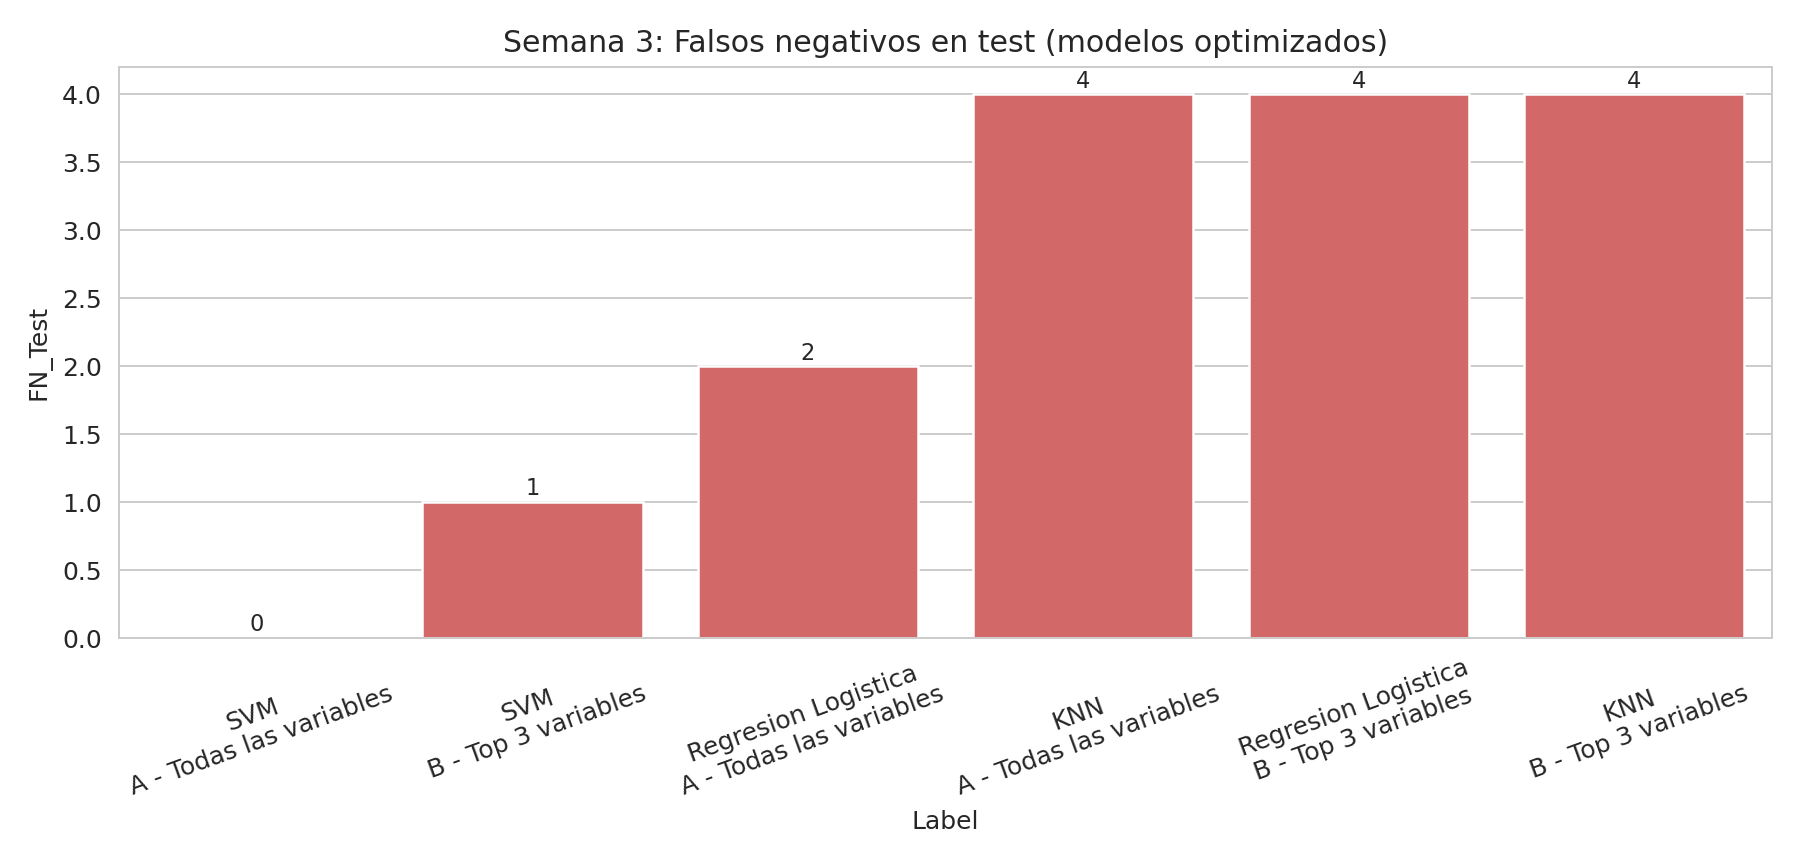
\includegraphics[width=0.9\textwidth]{figures/s3_fn_optimizado.png}
\caption{Falsos negativos en modelos optimizados. SVM-A: FN=0 (óptimo clínicamente).}
\label{fig:fn_optimizado}
\end{figure}

\begin{figure}[H]
\centering
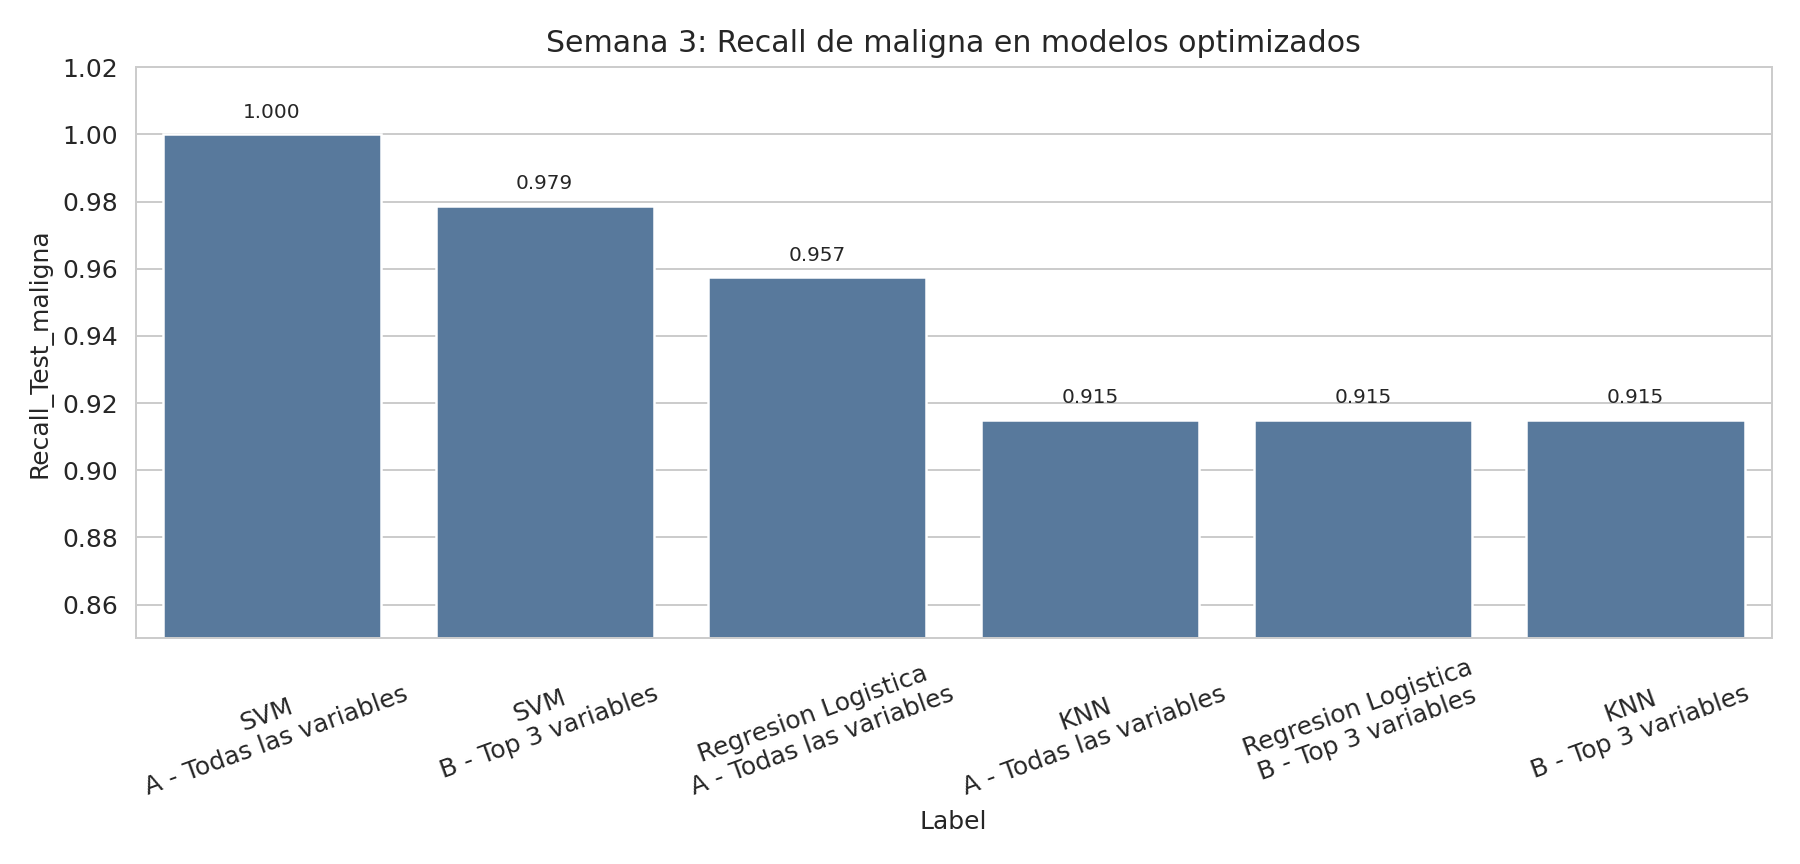
\includegraphics[width=0.9\textwidth]{figures/s3_recall_optimizado.png}
\caption{Recall de clase maligna en modelos optimizados. SVM-A: 100\% de sensibilidad.}
\label{fig:recall_optimizado}
\end{figure}

\subsection{Matriz de confusión del modelo final}

\begin{table}[H]
\centering
\caption{Matriz de confusión: SVM optimizado en Escenario A (test set, N=135)}
\renewcommand{\arraystretch}{1.3}
\begin{tabular}{l|cc|c}
\toprule
 & \textbf{Pred. Benigno (2)} & \textbf{Pred. Maligno (4)} & \textbf{Total Real} \\
\midrule
\textbf{Real Benigno (2)} & \cellcolor{lightgray}83 & \cellcolor{malignored!30}5 & 88 \\
\textbf{Real Maligno (4)} & \cellcolor{lightgray}0 & \cellcolor{benigngreen!30}47 & 47 \\
\midrule
\textbf{Total Predicho} & 83 & 52 & 135 \\
\bottomrule
\end{tabular}
\end{table}

\subsection{Justificación de la selección de SVM-A}

La selección de SVM optimizado en Escenario A fue fundamentada en:

\begin{enumerate}[leftmargin=1.4cm]
\item \textbf{Recall maligna máximo:} 1.0000 (todos los malignos detectados sin excepción)
\item \textbf{Falsos negativos mínimo absoluto:} FN = 0 (ningún maligno omitido)
\item \textbf{Consistencia CV-Test:} rendimiento replicable en validación cruzada
\item \textbf{Coherencia clínica:} alineado con el objetivo establecido de minimizar riesgo de falsos negativos
\end{enumerate}

\textbf{Trade-off explícito aceptado:}
\begin{itemize}[leftmargin=1.4cm]
\item Frente a LR-A optimizada: SVM-A evita 2 falsos negativos adicionales a cambio de 2 falsos positivos más
\item En contexto clínico: evaluaciones adicionales (FP) son siempre preferibles a diagnósticos tardíos (FN)
\end{itemize}

% ─────────────────────────────────────────────
\section{Semana 4: Interpretabilidad, Análisis de Errores y Cierre Técnico}
% ─────────────────────────────────────────────

\subsection{Desafío de interpretabilidad en SVM-RBF}

SVM con kernel RBF no ofrece importancias de variables directas. Para resolverlo sin alterar el modelo final, se aplicó una estrategia de \textbf{interpretabilidad triangulada}:

\begin{enumerate}[leftmargin=1.4cm]
\item Entrenar Random Forest (extrae importancias por impureza)
\item Entrenar Regresión Logística (extrae coeficientes estandarizados)
\item Promediar rankings de ambos modelos
\end{enumerate}

La convergencia entre modelos distintos valida la importancia genuina de variables.

\subsection{Ranking combinado de importancia}

\begin{table}[H]
\centering
\caption{Importancia de variables: RF $\times$ LR combinado}
\small
\renewcommand{\arraystretch}{1.15}
\begin{tabular}{lcccc}
\toprule
\textbf{Posición} & \textbf{Variable} & \textbf{RF rank} & \textbf{LR rank} & \textbf{Promedio} \\
\midrule
\rowcolor{bestrow}
1 & Bare Nuclei & 3 & 1 & 2.0 \\
\rowcolor{bestrow}
2 & Uniformity of Cell Shape & 2 & 3 & 2.5 \\
\rowcolor{bestrow}
3 & Uniformity of Cell Size & 1 & 6 & 3.5 \\
\midrule
4 & Clump Thickness & 7 & 2 & 4.5 \\
4 & Bland Chromatin & 5 & 4 & 4.5 \\
\midrule
6 & Marginal Adhesion & 8 & 5 & 6.5 \\
6 & Single Epithelial Cell Size & 4 & 9 & 6.5 \\
6 & Normal Nucleoli & 6 & 7 & 6.5 \\
\midrule
9 & Mitoses & 9 & 8 & 8.5 \\
\bottomrule
\end{tabular}
\normalsize
\end{table}

\textbf{Hallazgo:} las tres variables de máxima importancia (Bare Nuclei, Uniformities) concentran el poder predictivo. Esto confirma coherencia con hipótesis H1 de Semana 1.

\subsection{Análisis de falsos positivos}

Con FN=0 (resultado óptimo), el análisis se enfoca en los 5 falsos positivos para caracterizar dónde y por qué falla el modelo.

\textbf{Perfil de los FP:}

\begin{table}[H]
\centering
\caption{Perfil citológico: FP vs. benignos normales vs. malignos verdaderos}
\small
\renewcommand{\arraystretch}{1.15}
\begin{tabular}{lccc}
\toprule
\textbf{Variable} & \textbf{FP (media)} & \textbf{TN (media)} & \textbf{TP (media)} \\
\midrule
Clump Thickness & 3.60 & 2.69 & 5.98 \\
Uniformity of Cell Size & 3.60 & 1.54 & 6.83 \\
Uniformity of Cell Shape & 3.20 & 1.60 & 6.70 \\
Marginal Adhesion & 2.80 & 1.54 & 5.81 \\
Single Epithelial Cell Size & 5.40 & 1.82 & 6.70 \\
\textbf{Bare Nuclei} & \textbf{4.20} & 1.77 & 7.40 \\
Bland Chromatin & 3.80 & 1.54 & 6.72 \\
Normal Nucleoli & 3.40 & 1.71 & 5.68 \\
Mitoses & 1.40 & 1.05 & 1.53 \\
\bottomrule
\end{tabular}
\normalsize
\end{table}

\textbf{Interpretación:} los FP son \textbf{benignos con fenotipo citológico atípico}, ubicados en la zona intermedia. El modelo los clasifica como malignos debido a su proximidad a la frontera de decisión. Clínicamente: evaluaciones adicionales son el costo aceptado de máxima sensibilidad.

\begin{figure}[H]
\centering
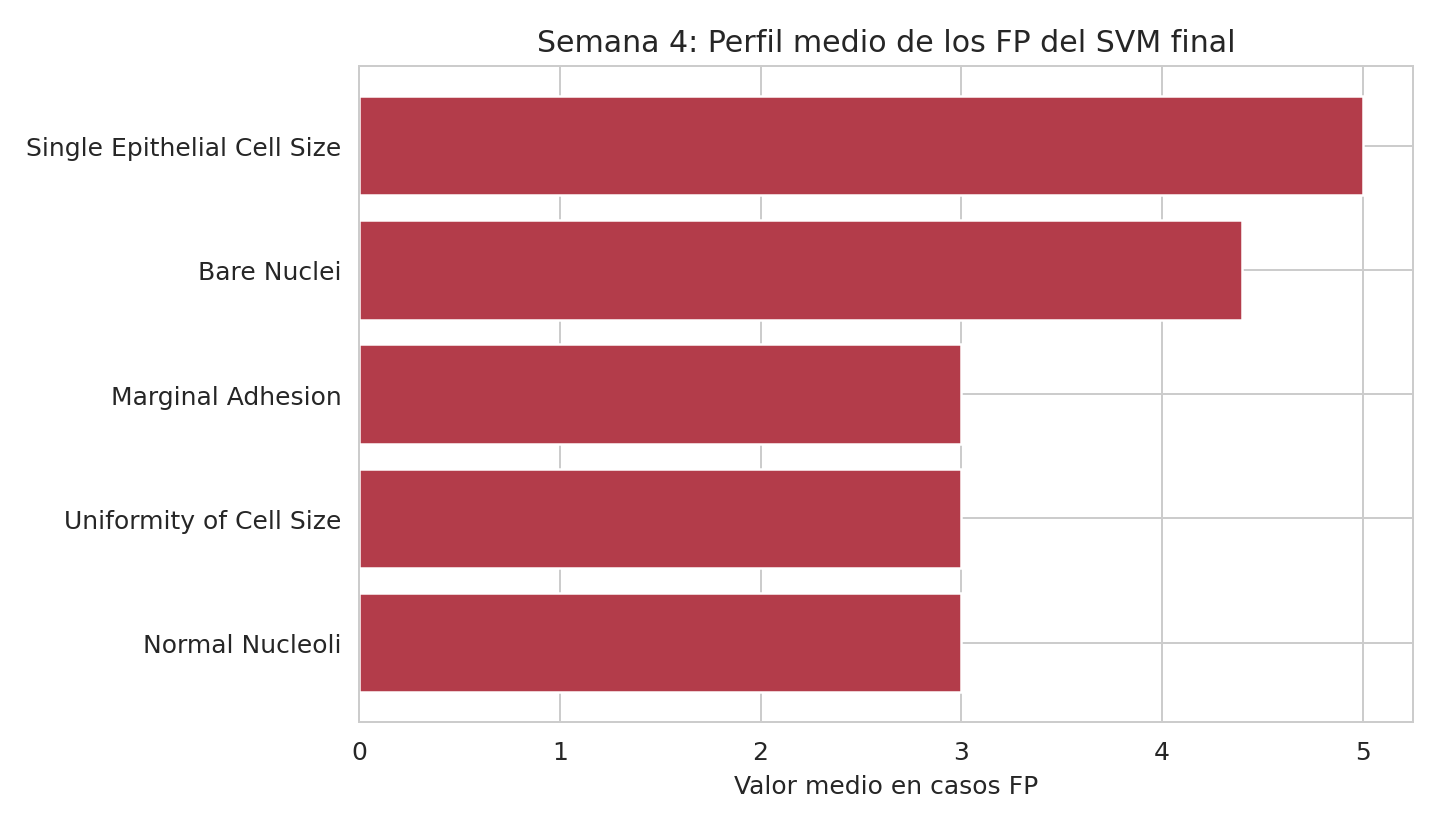
\includegraphics[width=0.9\textwidth]{figures/s4_fp_perfil_medio.png}
\caption{Perfil de falsos positivos: posición intermedia entre benignos normales y malignos.}
\label{fig:fp_perfil}
\end{figure}

\subsection{Comparación de trade-offs clínicos}

\begin{table}[H]
\centering
\caption{Trade-off SVM-A vs. LR-A en test set}
\renewcommand{\arraystretch}{1.3}
\begin{tabular}{lcccccc}
\toprule
\textbf{Modelo} & \textbf{TP} & \textbf{FN} & \textbf{FP} & \textbf{Recall} & \textbf{Precision} & \textbf{Especificidad} \\
\midrule
\rowcolor{bestrow}
SVM-A & 47 & 0 & 5 & 1.0000 & 0.9038 & 0.9432 \\
LR-A & 45 & 2 & 3 & 0.9574 & 0.9375 & 0.9659 \\
\midrule
\textbf{Diferencia} & +2 & -2 & +2 & +0.0426 & -0.0337 & -0.0227 \\
\bottomrule
\end{tabular}
\end{table}

\textbf{Lectura clínica:} SVM-A evita 2 falsos negativos (malignos no detectados) a cambio de 2 falsos positivos (biopsias adicionales). En oncología, este trade-off es clínicamente aceptable.

% ─────────────────────────────────────────────
\section{Discusión integrada y coherencia del proyecto}
% ─────────────────────────────────────────────

\subsection{Narrativa técnica completa}

El proyecto mantiene coherencia metodológica a lo largo de las 4 semanas:

\begin{enumerate}[leftmargin=1.4cm]
\item \textbf{Semana 1:} Identifica variables relevantes mediante análisis exploratorio y define hipótesis guiadoras.
\item \textbf{Semana 2:} Implementa escenarios y establece baselines, confirmando ventaja preliminar de SVM.
\item \textbf{Semana 3:} Valida rigorosamente, optimiza hiperparámetros, y selecciona SVM-A con justificación cuantitativa.
\item \textbf{Semana 4:} Explica qué aprende el modelo e interpreta dónde falla, cerrando trazabilidad completa.
\end{enumerate}

\subsection{Fortalezas técnicas del proyecto}

\begin{enumerate}[leftmargin=1.4cm]
\item \textbf{Control experimental homogéneo:} protocolo idéntico para todos los modelos (5-Fold CV, mismos datos, mismo split).
\item \textbf{Métrica clínicamente informada:} Recall maligna como objetivo, no Accuracy genérico.
\item \textbf{Justificación cuantitativa:} todas las decisiones respaldadas por datos y trade-offs explícitos.
\item \textbf{Reproducibilidad:} semillas de aleatoriedad controladas (\texttt{random\_state=42}), datos y resultados archivados.
\item \textbf{Trazabilidad completa:} linkage entre semanas sin contradicciones metodológicas.
\end{enumerate}

\subsection{Limitaciones identificadas}

\begin{enumerate}[leftmargin=1.4cm]
\item \textbf{Tamaño de dataset:} 675 muestras es moderado; validación externa en cohortes mayores es recomendada.
\item \textbf{Interpretabilidad indirecta de SVM-RBF:} se usaron modelos proxy (RF, LR) para inferir patrones.
\item \textbf{Persistencia de FP en frontera:} 5 casos son benignos con fenotipo atípico, difíciles de distinguir.
\item \textbf{Sin validación externa:} todas las métricas están en datos del mismo dataset; validación cruzada en otro centro es necesaria.
\end{enumerate}

% ─────────────────────────────────────────────
\section{Conclusiones}
% ─────────────────────────────────────────────

\begin{enumerate}[leftmargin=1.4cm]
\item El objetivo principal del proyecto se cumplió: diseñar y seleccionar un modelo de clasificación con mínima omisión de malignos.

\item \textbf{SVM optimizado en Escenario A} fue el único candidato que logró \textbf{FN=0 en test bajo protocolo comparable y riguroso}.

\item La selección no se basó en Accuracy aislada, sino en \textbf{criterio clínico explícito}: priorizar recall maligna y minimizar riesgo de diagnósticos tardíos.

\item Las variables más influyentes del modelo final son \textbf{Bare Nuclei} y las \textbf{uniformidades celulares}, convergentes con hallazgos de Semana 1.

\item El cierre de interpretabilidad y errores en Semana 4 fortalece la \textbf{defendibilidad técnica y clínica del proyecto}.

\item El modelo es \textbf{implementable en contexto clínico} con protocolos de segunda revisión para positivos, asegurando uso responsable.
\end{enumerate}

% ─────────────────────────────────────────────
\section{Recomendaciones finales}
% ─────────────────────────────────────────────

\begin{enumerate}[leftmargin=1.4cm]
\item \textbf{Mantener SVM-A} como modelo productivo mientras el objetivo siga siendo minimizar falsos negativos en diagnósticos de cáncer.

\item \textbf{Reportar siempre metricas multi-dimensionales:} Recall maligna, FN absoluto, Precision, AUC, FP, especificidad. Nunca reportar una métrica única.

\item \textbf{Implementar protocolo de segundo análisis:} toda predicción de malignidad debe pasar por validación clínica adicional.

\item \textbf{Monitoreo en producción:} llevar registro sistemático de FP confirmados en clínica para detectar sesgos sistemáticos.

\item \textbf{Calibración de umbral futuro:} si costos clínicos locales cambian, recalibrar el threshold sin reentrenar.

\item \textbf{Validación externa:} antes de despliegue fuera del contexto académico, validar en cohorte independiente de otro centro clínico.

\item \textbf{Auditoría documentada:} mantener esta narrativa completa como referencia permanente para futuras mejoras o investigaciones.
\end{enumerate}

% ─────────────────────────────────────────────
\section{Estructura de entregables del proyecto}
% ─────────────────────────────────────────────

\subsection{Documentación}

\begin{itemize}[leftmargin=1.4cm]
\item \textbf{README.md:} descripción ejecutiva del proyecto y guía de archivos
\item \textbf{docs/01\_Semana\_01\_Informe.tex:} informe de EDA
\item \textbf{docs/02\_Semana\_02\_Informe.tex:} informe de preparación de datos y baselines
\item \textbf{docs/03\_Semana\_03\_Informe.tex:} informe de validación y optimización
\item \textbf{docs/04\_Semana\_04\_Informe.tex:} informe de interpretabilidad y análisis de errores
\item \textbf{docs/05\_Informe\_Final\_Proyecto.tex:} este documento (integración de semanas)
\end{itemize}

\subsection{Notebooks técnicos}

\begin{itemize}[leftmargin=1.4cm]
\item \textbf{notebook/01\_Semana\_01\_EDA.ipynb:} análisis exploratorio
\item \textbf{notebook/02\_Semana\_02\_PrepData\_Modelos\_Base.ipynb:} preparación y baselines
\item \textbf{notebook/03\_Semana\_03\_Validacion\_Diseno\_Experimental.ipynb:} CV, tuning, selección
\item \textbf{notebook/04\_Semana\_04\_Interpretabilidad\_Errores.ipynb:} interpretabilidad y análisis de errores
\end{itemize}

\subsection{Datos y resultados}

\begin{itemize}[leftmargin=1.4cm]
\item \textbf{data/Datos.csv:} dataset original (683 registros)
\item \textbf{data/Datos\_limpio.csv:} dataset limpio (675 registros, con ID)
\item \textbf{data/Datos\_modelado.csv:} dataset para modelado (675 registros, sin ID)
\item \textbf{data/resultados\_semana3\_csv/:} tablas de CV, tuning, comparaciones y matrices
\item \textbf{data/resultados\_semana4\_csv/:} errores, comparaciones y ranking de importancia
\end{itemize}

\subsection{Figuras y gráficas}

\begin{itemize}[leftmargin=1.4cm]
\item \textbf{docs/figures/:} gráficas de EDA, métricas, errores e interpretabilidad
\end{itemize}

\end{document}
